\documentclass[conference]{IEEEtran}
\IEEEoverridecommandlockouts
\usepackage{cite}
\usepackage{amsmath,amssymb,amsfonts}
\usepackage{graphicx}
\usepackage{textcomp}
\usepackage{xcolor}
\usepackage[utf8]{inputenc}
\usepackage[T1]{fontenc}
\usepackage{booktabs}
\usepackage{array}
\usepackage{url}
\usepackage{microtype}

\begin{document}

\title{AI-Driven Dynamic Ambulance Routing and Hospital Selection System with Real-Time Traffic and Resource Awareness}

% Author block intentionally left empty; add names and affiliations here when decided.
\author{\IEEEauthorblockN{\hspace{0pt}}}

\maketitle

\begin{abstract}
Ambulance crews have to pick a hospital and a route for every patient, but the bed counts they can see are refreshed only now and then and never include ambulances already on the road. Independent ``nearest hospital with a bed'' choices therefore tend to pile ambulances onto the same hospital. We built a simulator of Bengaluru with 18 hospitals and fitted its travel times to 3,861 Mapbox typical-traffic samples; on 105 unseen routes the error is 11.3\% against 25.8\% before calibration. In this simulator we compared nearest-hospital rules, the scoring rule of our first prototype, a capacity-aware heuristic, a congestion-game assignment that provably converges, and a PPO policy. Every method was tuned on validation seeds and tested once on 50 new seeds per scenario. Accounting for ambulances already on the way cuts the mean time to bed by 12\% at an evening peak and 17\% in a surge, and removes 87--93\% of turn-aways. The equilibrium assignment is as fast as the tuned heuristic and has 10--20\% fewer rejections. PPO matched the heuristic but did not beat it. Beds and calls are simulated, so the results compare policies and do not predict real response times.
\end{abstract}

\begin{IEEEkeywords}
ambulance dispatch, hospital selection, congestion game, Nash equilibrium, reinforcement learning, real-time traffic
\end{IEEEkeywords}

\section{Introduction}
For every patient an ambulance crew must decide where to go and how to get there. The nearest hospital may have no free bed of the right kind, and the shortest road may be jammed. Crowded emergency departments go on diversion, which can push patients onto neighbouring hospitals~\cite{baan2025emergency}, and crowding has been linked to higher short-term mortality even for non-critical patients~\cite{eidsto2024emergency}. Longer response times are associated with lower survival in suspected cardiac arrest~\cite{janosikova2026logistic}, but the clock does not stop when the ambulance arrives, so we measure the time until the patient is actually in a bed. Hospital capacity and hospital choice are known to affect dispatch outcomes~\cite{xu2024emergency,fu2025modelling}, yet traffic data, bed counts and route advice usually come from separate places.

A further problem is herding. Published bed counts are updated every few minutes and do not include ambulances that are already driving to the hospital. If several crews each choose the nearest hospital that shows a free bed, they can all arrive together; some are turned away and have to detour. We study how much this costs and which dispatch rule copes best.

Our contributions are: (i) a simulator of Bengaluru with 18 hospitals whose travel times are fitted to real Mapbox traffic samples and checked on held-out routes; (ii) a congestion-game assignment for simultaneous dispatches, with a convergence proof and an empirical check; (iii) a comparison of simple rules, the equilibrium assignment and a PPO policy, all tuned on validation seeds and tested once on separate seeds; and (iv) a FastAPI service and a map-based dispatcher console.

\section{Literature Review}
AI-enabled emergency routing has grown quickly since 2020, using deep neural networks (DNNs)~\cite{selvan2025ambulance}, multi-agent reinforcement learning (MARL) for traffic-signal priority~\cite{olusanya2025multi}, and LSTM and ResNet models for ambulance detection~\cite{alruwaili2025lstm}. Reviews trace a path from classical VRP/TSP and static heuristics to adaptive learning with GPS, 5G and simulators such as SUMO~\cite{bajwa2025ai,tluli2024survey}. Related work covers dispatch toolkits~\cite{mappouras2025toolkit}, predictive placement and routing~\cite{nahata2024optimising}, edge-AI route recommendation~\cite{ahmed2023edge}, congestion prediction~\cite{pratyusha2025edge} and deep reinforcement learning for vehicle routing under uncertainty~\cite{kadyrov2025deep}. Reinforcement learning has also been applied to redeploying ambulances~\cite{tluli2024dynamic}, to allocating resources in mass-casualty incidents~\cite{murare2025abms} and to healthcare operations more broadly~\cite{wu2025reinforcement}. The gaps most often reported are the lack of city-scale implementations, of triage- or survival-based rewards, of interoperability between agencies, of bias mitigation and of clinical outcome evaluation (Table~\ref{tab1}).

\begin{table*}[t]
\caption{Summary of key studies on AI methods for emergency routing}\label{tab1}
\scriptsize
\centering
\begin{tabular}{p{2.3cm}p{3cm}p{5.2cm}p{2.8cm}p{3cm}}
\toprule
\textbf{Authors} & \textbf{AI technique} & \textbf{Evolution} & \textbf{Limitation} & \textbf{Gap / future work} \\
\midrule
Selvan et al.\ \cite{selvan2025ambulance} & DNN for dynamic route optimisation & From VRP/TSP baselines to real-time ML with GPS and traffic data & High-dimensional data & Rerouting without retraining \\
Talukdar \cite{talukdar2024real} & IoT sensors, GPS & From static routes to real-time IoT updates & Interoperability & Multi-agency data sharing \\
Bajwa \cite{bajwa2025ai} & ML/DL for geospatial routing; RL for dispatch & Synthesis of 424 studies, from detection to integrated AI-EMS with live traffic and hotspot forecasts & Ethical and regulatory hurdles & Cross-city benchmarks \\
Olusanya et al.\ \cite{olusanya2025multi} & MARL for signal and emergency priority control & Single-agent RL to decentralised multi-agent policies in SUMO & Sim-to-real gap & Real EMS fleet training \\
Alruwaili et al.\ \cite{alruwaili2025lstm} & LSTM + ResNet18 ambulance detection & CV-based detection extended to audio-visual fusion and pathfinding for EMS corridors & Needs dense sensor coverage & City-scale deployment \\
Jiang et al.\ \cite{jiang2022deep} & Deep RL with attention and GRU & From ant-colony heuristics to learned policies for changing demand & Logistics, not medical EMS & Deployment under uncertainty \\
\bottomrule
\end{tabular}
\end{table*}

The closest work couples hospital choice with game-theoretic or simulation models. Fu et al.~\cite{fu2025modelling} combine a game-theoretic model with discrete-event simulation to study hospital strategies in city-scale dispatching, Xu et al.~\cite{xu2024emergency} recommend dispatches using simulation based on bed availability, Bhatia et al.~\cite{bhatia2024enhancing} apply game-theoretic optimisation to a smart-ambulance system, and Sutherland and Chakrabortty~\cite{sutherland2023optimal} route by patient severity. As far as we know, our study differs in that it isolates the effect of bed data that are stale and blind to in-flight ambulances, calibrates travel times to real traffic samples, backs the equilibrium step with a potential-function argument, and reports learned and hand-designed policies under the same tuning budget, including where the learned one falls short. The cited works pursue different objectives and use different data, so these comparisons are qualitative.

\section{Problem and Methods}
\subsection{Setting}
Let $\mathcal{H}$ be the hospitals ($|\mathcal{H}|=18$). Each has a general and an ICU bed pool $p$, with capacity $C_{h,p}$ and true occupancy $O_{h,p}(t)$. Dispatchers see only the published free count $F_{h,p}(t)$, a copy of $C_{h,p}-O_{h,p}$ refreshed every $\Delta=5$ minutes (bed availability as a dispatch input is studied in~\cite{xu2024emergency}). Let $L_{h,p}(t)$ be the number of ambulances sent to $(h,p)$ that have not yet arrived. The coordinator knows $L$, but $F$ does not include it.

Request $i$ arrives at time $t_i$ at location $x_i$ and needs pool $p_i$. Requests within the same two-minute window are decided together. The planner estimates the travel time $\tau_{ih}$; the real trip takes $\tau_{ih}\varepsilon$ with $\ln\varepsilon\sim\mathcal{N}(-\sigma^2/2,\sigma^2)$, which has mean one. On arrival the patient is admitted if $O_{h,p_i}<C_{h,p_i}$. Otherwise the ambulance is \emph{rejected}: after a five-minute handover delay it drives to the nearest untried hospital that shows a free bed (a \emph{diversion}), and after four diversions the patient waits 60 minutes. The main metric is the time to bed $D_i=t^{\mathrm{admit}}_i-t_i$ (mean and 95th percentile). We also report rejections per episode, the share of patients diverted, and Jain's fairness index of dispatches per bed across hospitals.

\subsection{Baselines and capacity heuristic}
\emph{Nearest} picks $\arg\min_h\tau_{ih}$ and ignores beds; \emph{nearest+beds} restricts the choice to hospitals with $F_{h,p_i}>0$; the \emph{prototype rule} is the scoring formula of our first prototype, $0.6\,\tau_{ih}[\mathrm{s}]+0.4\cdot1000/F_{h,p_i}$. The \emph{capacity heuristic} also counts ambulances already on the road. With effective free beds $E_h=F_{h,p_i}-L_{h,p_i}$ it scores $s_{ih}=\tau_{ih}+w/(1+\max(E_h,0))$ over hospitals with $E_h>0$ (nearest if there are none) and updates $L$ after each assignment in a batch.

\subsection{Equilibrium coordination}
\label{sec:nash}
Herding of this kind is the classic setting of congestion and selfish-routing games~\cite{rosenthal1973class}. Within a batch, request $i$ chooses a hospital and so a resource $r=(h,p_i)$. Let $n_r(a)$ be the number of batch requests assigned to $r$ under assignment $a$ and $\ell_r=L_{h,p_i}$. The cost of $i$ is
\begin{equation}
c_i(a)=\tau_{i,h(i)}+\beta\left(\frac{\ell_r+n_r(a)}{\max(F_r,1)}\right)^{\gamma}+\kappa\,\mathbf{1}[F_r\le 0],
\label{eq:cost}
\end{equation}
with $\beta>0$, $\gamma\ge1$ and a large constant $\kappa$. The second term charges for loading a resource beyond its published capacity. We start from a greedy assignment in arrival order and then let requests, in random order, switch to their cheapest hospital whenever that lowers their own cost by more than $10^{-9}$, repeating until nobody moves (at most 100 rounds).

\textbf{Proposition 1.} This best-response procedure ends at a pure Nash equilibrium.

\emph{Proof sketch.} Define $\Phi(a)=\sum_i\tau_{i,h(i)}+\sum_r\sum_{k=1}^{n_r(a)}\big[\beta\big(\tfrac{\ell_r+k}{\max(F_r,1)}\big)^{\gamma}+\kappa\mathbf{1}[F_r\le0]\big]$. When request $i$ moves from $r$ to $r'$, only the last load term of $r$ is removed and one new load term of $r'$ is added, and the travel term changes by the difference in $\tau$. These are exactly the changes in $i$'s own cost, so $\Phi(a')-\Phi(a)=c_i(a')-c_i(a)$. Every improving move therefore lowers $\Phi$ strictly. With finitely many assignments the process must stop, and a state with no improving move is a pure Nash equilibrium. This is Rosenthal's argument for congestion games~\cite{rosenthal1973class}. \hfill$\square$

Unit tests also confirm on random instances that no request can gain by switching alone.

\subsection{PPO policy}
\label{sec:ppo}
We trained a policy with Proximal Policy Optimization (PPO)~\cite{schulman2017proximal} using the Stable-Baselines3 library. For each request the observation describes the 12 nearest hospitals: scaled ETA, log free beds, free fraction, in-flight load over free beds, the clipped difference $(F-L)/20$, an overflow flag and the rank. Five global values are added (pool, time of day as sine and cosine, requests left in the batch, log of city-wide effective free beds), giving 89 inputs. The action picks one of the 12 candidates, and requests in a batch are handled one at a time so the policy sees the load created by its own earlier choices.

The training reward is $-\tau/10-1.5\cdot\mathbf{1}[\text{overflow}]-0.3\min(\text{load}/(\text{free}+1),3)$, where overflow means the true free beds are already covered by ambulances on the way. It is used only for training; every evaluation uses the real time to bed. Episodes sample the three scenarios in Table~\ref{tab:data} uniformly with seeds disjoint from validation and test. The network has two hidden layers of 128 units and is trained for $10^6$ steps (learning rate $10^{-4}$ with decay, clip 0.1, entropy coefficient 0.005). The network is warm-started by behaviour cloning of the capacity heuristic (150 episodes) and then fine-tuned with PPO. We trained three seeds and chose one on validation seeds only.

\subsection{System}
\label{sec:system}
A FastAPI service (Fig.~\ref{fig:arch}) exposes the hospital list, bed updates, single-ambulance selection (\texttt{/route}, \texttt{/route/drl}), batch assignment at equilibrium (\texttt{/assign}) and route lookup. If PPO is unavailable the service falls back to the equilibrium solver and then to the heuristic. Routing tries Mapbox (\texttt{driving-traffic}), then OSRM, then the calibrated built-in model, and returns GeoJSON with distance and duration. The dispatcher console (Fig.~\ref{fig:console}) shows incidents on a live-traffic map with the recommended hospital, route and ETA, and supports multi-ambulance assignment and hospital-side bed updates.

\begin{figure}[t]
\centering
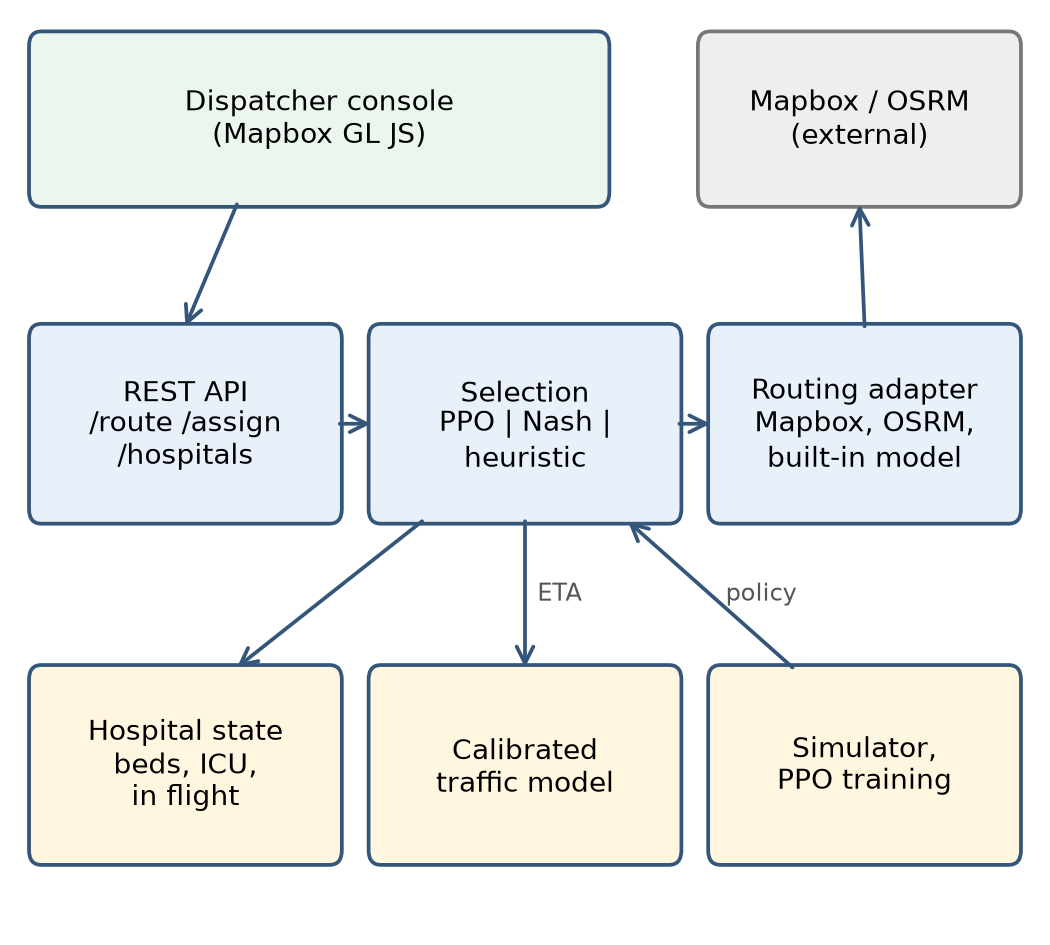
\includegraphics[width=\columnwidth]{fig_architecture.png}
\caption{Architecture of the implemented service.}
\label{fig:arch}
\end{figure}

\begin{figure}[t]
\centering
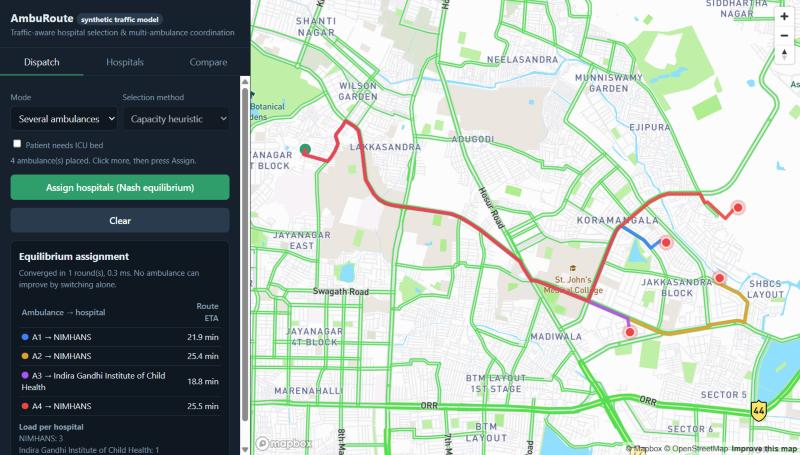
\includegraphics[width=0.95\columnwidth]{fig_console.jpg}
\caption{Dispatcher console with four ambulances assigned at an equilibrium and Mapbox routes.}
\label{fig:console}
\end{figure}

\section{Experimental Setup}
\subsection{Data and what is simulated}
Table~\ref{tab:data} separates real inputs from simulated ones. The results compare policies under these assumptions; they are not forecasts of real response times.

\begin{table}[t]
\caption{Data provenance and scenarios}
\label{tab:data}
\centering\scriptsize
\begin{tabular}{p{2.1cm}p{1.2cm}p{4.2cm}}
\toprule
Item & Status & Note \\
\midrule
Hospitals, coordinates, bed totals & Real table & 18 hospitals; 3 missing bed counts set to the median; two non-emergency hospitals removed \\
ICU beds & Synthetic & 8\% of beds, at least 4 \\
Bed occupancy & Simulated & Starts at 88--99\%, then random admissions and discharges \\
Ambulance calls & Simulated & Poisson, uniform over the city, 25\% need ICU \\
Travel times & Calibrated & Fitted to Mapbox typical traffic \\
Ambulance speed-up & Assumed & 1.25 over car times \\
\midrule
Scenarios & & Off-peak 0.5 calls/min, 120 min, 13:00; evening peak 1.2/min, 120 min, 17:30; surge 2.5/min, 60 min, 18:00 \\
\bottomrule
\end{tabular}
\end{table}

\subsection{Traffic calibration}
\label{sec:traffic}
Our first simulator used a hand-made speed curve. To replace it with real data we queried the Mapbox Directions API (\texttt{driving-traffic} with \texttt{depart\_at}) for 360 origin--destination pairs, half from random city points to a random hospital and half between hospitals, at 11 departure times from 00:00 to 22:30 on a weekday, and recorded \texttt{duration\_typical}. After dropping pairs shorter than 0.5\,km, 351 pairs and 3,861 samples remained. We split by pair, 70/30, so the 105 test pairs were never seen in fitting. A linear form (slope per hour plus intercept) was compared with a power law $\text{time}=\exp(c_{\text{hour}})\,d^{p}$ in straight-line distance $d$ by five-fold cross-validation on training pairs only. The power law won (12.3\% against 17.0\% error) and was scored once on the held-out pairs (Table~\ref{tab:traffic}, Fig.~\ref{fig:traffic}). The spread of the held-out residuals ($0.14$ in log units) sets the noise of simulated trips. Mapbox returns car times, so the 1.25 ambulance speed-up is an assumption, which we vary later.

\begin{table}[t]
\caption{Travel-time models against Mapbox typical traffic}
\label{tab:traffic}
\centering\footnotesize
\resizebox{\columnwidth}{!}{%%TAB:tab_traffic_small%%}
\end{table}

\begin{figure}[t]
\centering
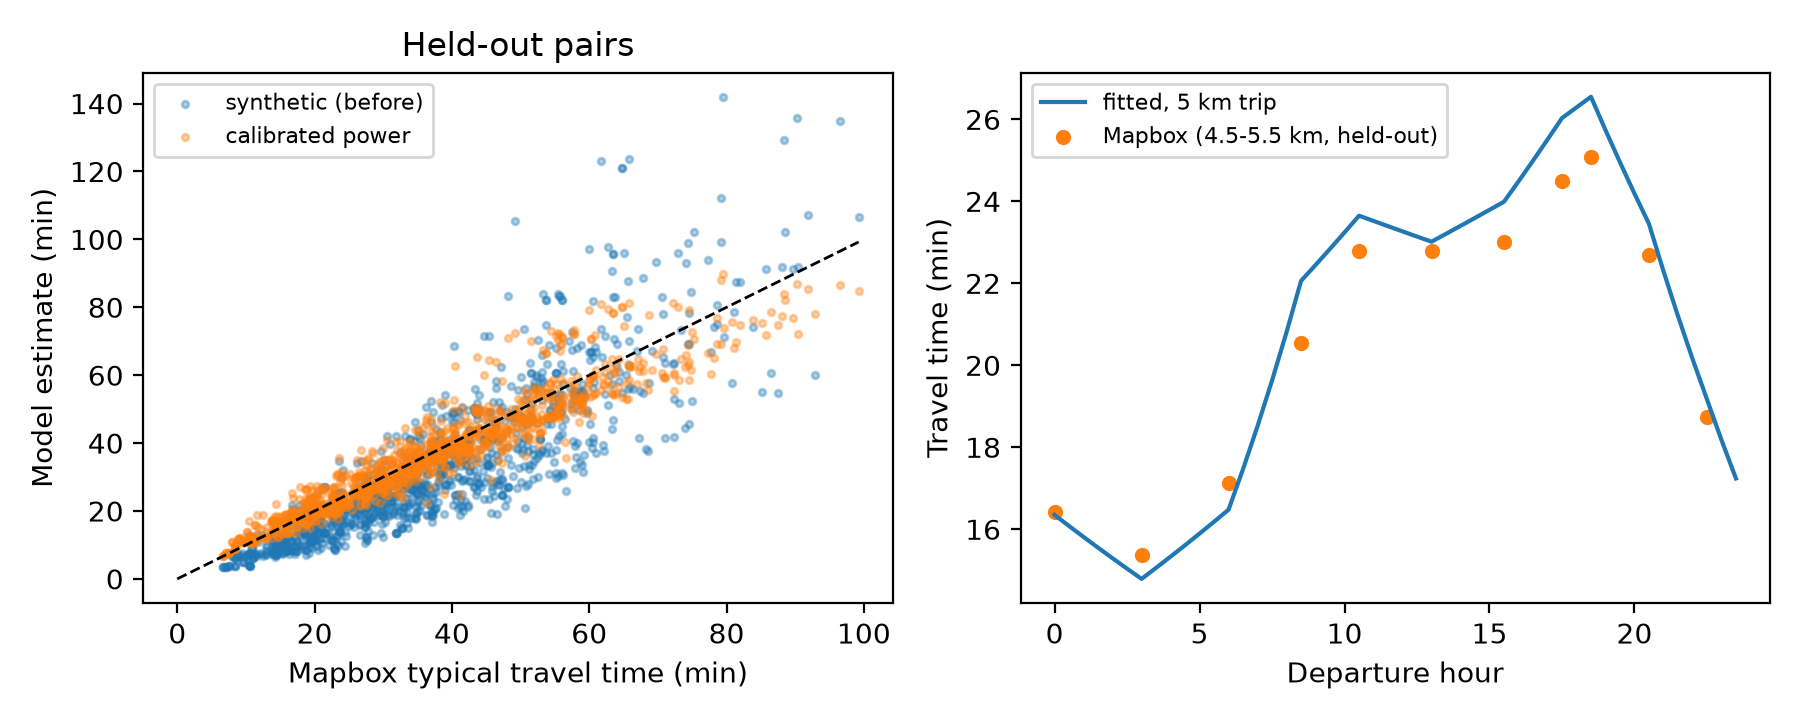
\includegraphics[width=\columnwidth]{fig_traffic_calibration.png}
\caption{Left: model against Mapbox on held-out pairs. Right: fitted profile for a 5\,km trip with held-out observations.}
\label{fig:traffic}
\end{figure}

\subsection{Protocol}
Seeds form three disjoint sets: training ($\ge10^5$), validation (500--529) and test (1000--1049). The hand-designed policies were tuned on validation seeds over $w\in\{5,10,20,30,50,80\}$ and $\beta\in\{5,10,20,30,45\}$, $\gamma\in\{1,2\}$, so they had the same tuning opportunity as PPO. Everything was then run once on the 50 test seeds per scenario. We report means with 95\% bootstrap intervals (5,000 resamples over seeds) and compare policies on identical seeds with the Wilcoxon signed-rank test, using Holm correction within each scenario and metric.

\section{Results}
\label{sec:results}
\subsection{Main comparison}
Table~\ref{tab:main} gives the test results. The biggest effect comes from counting ambulances that are already on the way. Compared with nearest-hospital dispatch, the capacity heuristic and the equilibrium assignment shorten the mean time to bed by about 5\% off-peak, 12\% at the evening peak (3.1 min for the equilibrium policy, 95\% CI $[-3.7,-2.6]$) and 17\% in the surge (4.8 min, $[-5.7,-4.0]$); all six comparisons have Holm $p<0.001$ (Table~\ref{tab:tests}). The 95th percentile drops from 62.9 to 39.9 min at peak and from 74.2 to 41.5 min in the surge. Rejections per episode fall from 30.1 to 2.8 (peak) and from 46.8 to 5.6 (surge), and the share of ICU patients who are diverted falls from 37\% to 4\% and from 42\% to 5\%. The old prototype rule beats nearest-hospital dispatch but trails the capacity-aware policies by 0.9--1.0 min (4\%) at peak and 2.3 min (9\%) in the surge; off-peak the differences are not significant.

\begin{table*}[t]
\caption{Test results on 50 held-out seeds per scenario: mean time to bed in minutes with 95\% bootstrap CI, 95th percentile, rejections per episode, share of patients diverted, and Jain index}
\label{tab:main}
\centering\footnotesize
%%TAB:tab_main%%
\end{table*}

\begin{table}[t]
\caption{Paired differences in mean time to bed (key pairs)}
\label{tab:tests}
\centering\scriptsize
\resizebox{\columnwidth}{!}{%%TAB:tab_tests_small%%}
\end{table}

\subsection{Equilibrium assignment against the heuristic}
The two capacity-aware policies do not differ in mean time to bed (differences of $+0.01$, $-0.09$ and $-0.06$ min off-peak, peak and surge; all intervals contain zero; Holm $p\ge0.37$). They do differ elsewhere. The equilibrium assignment has fewer rejections at peak (2.8 against 3.5 per episode, $-20\%$, Holm $p=0.010$) and in the surge (5.6 against 6.2, $-10\%$, $p=0.025$), and a more even load (Jain 0.51 against 0.48, and 0.52 against 0.47). So it buys fewer turn-aways and a convergence guarantee, not faster dispatch.

Best-response dynamics converged in all 4,239 batches of the peak and surge scenarios (2,747 and 1,492), after 1.00 and 1.02 rounds on average and at most 2 and 3. Most batches are small, so the greedy start is already close to an equilibrium. Table~\ref{tab:beta} varies the congestion weight. With $\beta=0$ the policy is nearest+beds. Mean time to bed is lowest for $\beta$ between 10 and 20, while rejections keep falling as $\beta$ grows, at the price of longer trips. We used $\beta=10$, $\gamma=2$, chosen on validation seeds.

\begin{table}[t]
\caption{Effect of the congestion weight $\beta$ on mean time to bed (min) and rejections per episode}
\label{tab:beta}
\centering\footnotesize
%%TAB:tab_beta_small%%
\end{table}

\subsection{PPO}
PPO did not improve on the tuned heuristic. On validation seeds the three trained seeds scored 21.82, 21.83 and 22.07 min against 21.51 for the heuristic, and we used the best one (retraining gives slightly different policies, so the seeds differ by up to 0.25 min). On the test seeds it is level with the heuristic off-peak ($-0.01$ min, Holm $p=0.81$) and slower at peak (0.21 min, $p=0.044$) and in the surge (0.53 min, $p<0.001$), that is 0.9--2.3\%, with 57\% and 79\% more rejections at peak and surge. It does beat the old prototype rule at peak ($-0.70$ min, 36 of 50 seeds, $p=0.0004$, Bonferroni-adjusted for three comparisons $0.001$) and in the surge ($-1.73$ min, 42 of 50, $p<0.001$), shows no difference off-peak ($-0.12$ min, $p=0.38$), and beats nearest-hospital dispatch by 11\% and 15\%. Earlier attempts on a first, synthetic-traffic version of the simulator did worse: learning from scratch with fewer inputs was 8--9\% behind the heuristic, and a 12-candidate variant with a herding penalty but no warm start was about 5\% behind on validation seeds. In this setting a learned policy reaches heuristic-level quality and stops there. Reinforcement learning has been reported to help with ambulance redeployment~\cite{tluli2024dynamic}; for the hospital choice studied here there appears to be less room for a learned policy.

\subsection{Sensitivity}
Table~\ref{tab:robust} varies conditions that dispatchers do not control. Letting bed data age to 30 minutes hurts the heuristic by 0.72 min at peak and 1.29 min in the surge ($p<0.001$) and the equilibrium policy by 0.28 and 0.98 min. At that refresh interval the equilibrium policy is ahead of the heuristic at peak (0.44 min, Bonferroni $p=0.024$) but not significantly in the surge (0.30 min, $p=0.18$); at 1--15 minutes the two are indistinguishable. We read this as a modest advantage for very stale data, not a general one.

Swapping the traffic-aware ETAs for free-flow ones, as in a traffic-service outage, changed mean time to bed by less than 0.25 min for both policies, because the ETAs mostly serve to rank hospitals and the ranking barely moves. The outage would still distort the ETA shown to the dispatcher, which is why routing falls back to OSRM and then to the built-in model. The ambulance speed-up changes absolute times a lot (equilibrium policy at peak: 28.0, 22.6 and 19.0 min for 1.0, 1.25 and 1.5) but not the comparison: it stays 12--13\% faster than nearest-hospital dispatch at peak and 14--17\% in the surge. Doubling or halving the trip noise moved its mean by less than 0.1 min. Deciding one request takes under 1 ms for every policy (about 0.04 ms for the heuristic, 0.08 ms for the equilibrium solver and 0.8 ms for PPO on a laptop CPU), while one Mapbox route request took about 0.5--0.7 s in our tests, so routing dominates latency.

\begin{table}[t]
\caption{Mean time to bed (min) under varied conditions, 50 test seeds. Near.\ = nearest, Heur.\ = capacity heuristic, Nash = equilibrium assignment}
\label{tab:robust}
\centering\scriptsize
\resizebox{\columnwidth}{!}{%%TAB:tab_robust_small%%}
\end{table}

\section{Discussion and Limitations}
Almost all of the gain over nearest-hospital dispatch comes from one ingredient, accounting for ambulances already heading to a hospital. The heuristic does it directly and the equilibrium step through the load term in~\eqref{eq:cost}. Refreshing beds every minute instead of every five improves the heuristic by only about 0.2 min, so there is little unused information for a learned policy to find. That fits PPO matching but not beating a tuned rule. It is an inference from this simulator, not a general statement about reinforcement learning for dispatch; richer problems with triage priorities or specialty capacity may leave more room.

The main limitations are these. Bed occupancy, ICU capacity and call locations are simulated, so the staleness study is only a proxy for real hospital feeds. Travel times follow typical traffic; incidents and day-to-day swings appear only as noise. The planner uses a fitted function of straight-line distance, while Mapbox supplies the final route and ETA. The ambulance speed-up is an assumption. Time to bed is a stand-in for clinical outcome, and we do not model triage or specialty capability, both of which earlier reviews list as open gaps~\cite{bajwa2025ai,tluli2024survey}. Several of the 18 hospitals are specialist centres (cardiac, chest, paediatric, neuro-psychiatric) that we treat as general receivers. The study covers one city. Finally, automated recommendations should support the dispatcher and not replace them, bed reports can be late or wrong, and a load-balancing equilibrium could disadvantage areas near busy hospitals, so a field study is needed before any deployment. No patient data were used.

\section{Conclusion}
We formalised hospital selection when bed data are stale and blind to ambulances already on the road, calibrated a simulator to 3,861 real traffic samples, and compared simple rules, an equilibrium assignment and PPO under the same tuning and held-out testing. Counting ambulances in flight shortened time to bed by 12\% at the evening peak and 17\% in a surge and removed most turn-aways. The equilibrium assignment matched the heuristic's speed with 10--20\% fewer rejections and an even load, and PPO reached the same level without exceeding it. The next steps are a live, authenticated hospital bed feed, incident-aware traffic, triage-weighted and specialty-aware objectives, and a field study with dispatchers.

\textbf{Availability.} The simulator, fitted traffic parameters, trained policies, experiment scripts and console are available at \textcolor{red}{[REPOSITORY URL TO BE ADDED]}. The raw Mapbox responses are not redistributed; the collection script regenerates them with the reader's own token. A single script regenerates every table and figure from the per-seed results.

\begin{thebibliography}{99}
\bibitem{selvan2025ambulance}
C. Selvan, B. H. Anwar, S. Naveen, and S. T. Bhanu, ``Ambulance route optimization in a mobile ambulance dispatch system using deep neural network (DNN),'' \emph{Sci. Rep.}, vol. 15, Art. no. 14232, 2025.

\bibitem{bajwa2025ai}
A. Bajwa, ``AI-based emergency response systems: A systematic literature review on smart infrastructure safety,'' SSRN 5171521, 2025.

\bibitem{olusanya2025multi}
O. Olusanya \emph{et al.}, ``Multi-agent reinforcement learning framework for autonomous traffic signal control in smart cities,'' \emph{Front. Mech. Eng.}, vol. 11, Art. no. 1650918, 2025.

\bibitem{alruwaili2025lstm}
M. Alruwaili \emph{et al.}, ``LSTM and ResNet18 for optimized ambulance routing and traffic signal control in emergency situations,'' \emph{Sci. Rep.}, vol. 15, Art. no. 6011, 2025.

\bibitem{mappouras2025toolkit}
S. Mappouras \emph{et al.}, ``A toolkit for ambulance dispatch and routing optimization using AI and GIS,'' in \emph{Proc. RSCy2025}, vol. 13816, pp. 361--367, SPIE, 2025.

\bibitem{pratyusha2025edge}
T. Pratyusha \emph{et al.}, ``Edge AI for smart traffic management: Real-time deep learning for congestion prediction and optimization,'' in \emph{Proc. ICMCTC}, pp. 1--4, IEEE, 2025.

\bibitem{kadyrov2025deep}
S. Kadyrov, A. Azamov, Y. Abdumajitov, and C. Turan, ``Deep reinforcement learning for dynamic vehicle routing with demand and traffic uncertainty,'' \emph{Oper. Res. Perspect.}, Art. no. 100351, 2025.

\bibitem{fu2025modelling}
X. Fu, V. Krzhizhanovskaya, A. Yakovlev, and S. Kovalchuk, ``Modelling diversity in hospital strategies in city-scale ambulance dispatching with coupled game-theoretic model and discrete-event simulation,'' \emph{J. Biomed. Inform.}, vol. 162, Art. no. 104777, 2025.

\bibitem{talukdar2024real}
C. Talukdar, ``Real-time routing in IoT networks for emergency response in smart cities,'' \emph{Risk Assess. Manag. Decis.}, vol. 1, no. 2, pp. 322--328, 2024.

\bibitem{tluli2024survey}
R. Tluli \emph{et al.}, ``A survey of machine learning innovations in ambulance services: Allocation, routing, and demand estimation,'' \emph{IEEE Open J. Intell. Transp. Syst.}, 2024.

\bibitem{nahata2024optimising}
H. Nahata, J. Dhaka, S. Soni, and V. GN, ``Optimising ambulance placement and routing using ML-driven predictive analytics for enhanced emergency response,'' in \emph{Proc. ICERCS}, pp. 1--7, IEEE, 2024.

\bibitem{xu2024emergency}
Y.-Y. Xu \emph{et al.}, ``The emergency medical service dispatch recommendation system using simulation based on bed availability,'' \emph{BMC Health Serv. Res.}, vol. 24, Art. no. 1513, 2024.

\bibitem{bhatia2024enhancing}
G. S. Bhatia \emph{et al.}, ``Enhancing emergency response: A smart ambulance system using game-building theory and real-time optimization,'' \emph{Int. J. Adv. Comput. Sci. Appl.}, vol. 15, no. 9, 2024.

\bibitem{ahmed2023edge}
S. T. Ahmed \emph{et al.}, ``An edge-AI-enabled autonomous connected ambulance-route resource recommendation protocol (ACA-R3) for eHealth in smart cities,'' \emph{IEEE Internet Things J.}, vol. 10, no. 13, pp. 11497--11506, 2023.

\bibitem{sutherland2023optimal}
M. Sutherland and R. K. Chakrabortty, ``An optimal ambulance routing model using simulation based on patient medical severity,'' \emph{Healthc. Anal.}, vol. 4, Art. no. 100256, 2023.

\bibitem{jiang2022deep}
H. Jiang, T. Guo, Z. Yang, and L. Zhao, ``Deep reinforcement learning algorithm for solving material emergency dispatching problem,'' \emph{Math. Biosci. Eng.}, vol. 19, pp. 10864--10881, 2022.

\bibitem{schulman2017proximal}
J. Schulman, F. Wolski, P. Dhariwal, A. Radford, and O. Klimov, ``Proximal policy optimization algorithms,'' arXiv:1707.06347, 2017.

\bibitem{rosenthal1973class}
R. W. Rosenthal, ``A class of games possessing pure-strategy Nash equilibria,'' \emph{Int. J. Game Theory}, vol. 2, no. 1, pp. 65--67, 1973.

\bibitem{baan2025emergency}
E. C. M. Baan-Kooman \emph{et al.}, ``Emergency department crowding in the Netherlands; evaluation of a real-time ambulance diversion dashboard,'' \emph{Int. J. Emerg. Med.}, vol. 18, no. 1, Art. no. 18, 2025.

\bibitem{eidsto2024emergency}
A. Eidst{\o} \emph{et al.}, ``Emergency department crowding increases 10-day mortality for non-critical patients: a retrospective observational study,'' \emph{Intern. Emerg. Med.}, vol. 19, no. 1, pp. 175--181, 2024.

\bibitem{janosikova2026logistic}
{\v L}. J{\'a}no{\v s}{\'\i}kov{\'a} \emph{et al.}, ``Logistic regression and simulation modelling to evaluate survival effects of EMS response time in suspected cardiac arrest,'' \emph{BMC Emerg. Med.}, vol. 26, no. 1, Art. no. 166, 2026.

\bibitem{tluli2024dynamic}
R. Tluli, A. Badawy, S. Salem, M. Hardan, S. Chauhan, and G. Alinier, ``A dynamic redeployment system for mobile ambulances in Qatar, empowered by deep reinforcement learning,'' in \emph{Proc. Int. Wireless Commun. Mobile Comput. Conf. (IWCMC)}, pp. 980--985, IEEE, 2024.

\bibitem{murare2025abms}
I. Murare{\c t}u, A. Vultureanu-Albi{\c s}i, S. Ilie, and C. B{\u a}dic{\u a}, ``ABMS-driven reinforcement learning for dynamic resource allocation in mass casualty incidents,'' \emph{Future Internet}, vol. 17, no. 11, Art. no. 502, 2025.

\bibitem{wu2025reinforcement}
Q. Wu, J. Han, Y. Yan, Y.-H. Kuo, and Z.-J. M. Shen, ``Reinforcement learning for healthcare operations management: methodological framework, recent developments, and future research directions,'' \emph{Health Care Manag. Sci.}, vol. 28, no. 2, pp. 298--333, 2025.
\end{thebibliography}

\end{document}
